\chapter{Teoretická část}
\section{Suspendace}
Smyslem suspendace v mechanicky míchaných nádobách je udržení pevných částic ve vznosu tak, aby došlo ke zintenzivnění transportu hmoty a tepla mezi kapalinou a pevnou fází. Pro dosažení tohoto stavu je třeba systému dodat energii v podobě mechanické práce. K vykonání této práce se používají rozmanité typy mechanických míchadel, které jsou voleny podle konkretního charakteru dané úlohy. Dodaná energie poté vede k vytvoření turbulentního proudění, jenž uvede částice pevné fáze do vznosu a následně je rozptýlí v kapalině. Nutnou podmínkou pro zajištění tohoto vznosu je potřeba, aby výsledná vertikální složka síly působící na částici byla větší než tíhová síla zmenšená o sílu vztlakovou. Menší částice jejichž hustota je přibližně rovna hustotě kapalina se po dosažení suspenzních podmínek pohybují společně s kapalinou. Při nižších koncentracích pevné fáze se toto proudění chová spíše jako jednofázový tok. Naopak rychlost pohybu těžších částic se liší od rychlosti kapalné fáze, jenž musí na pevnou fázi působit větší silou k zabránění jejímu usazování. Výslednou kvalitu vzniklé suspenze ovlivňuje řada faktorů, kde mezi nejvýznamnější patří fyzikální vlastnosti, jak kapalné, tak pevné fáze, provozní podmínky a geometrie systému a míchadla.

\subsection{Stupně suspendace}
Nároky na homogenitu vsádky se liší dle konkretních provozních požadavků. Jedním z pojmů, který se používá k popisu míry homogenizace vsádky v mechanicky míchaných nádobách je stupeň suspendace. Obecně se rozlišují tři stupně suspendace: částečná, úplná a homogenní (obr. \ref{fig:typsus}). 
  
\begin{figure}[h!]
  \centering
  \subfloat[Částečná]{\label{fig:typ1}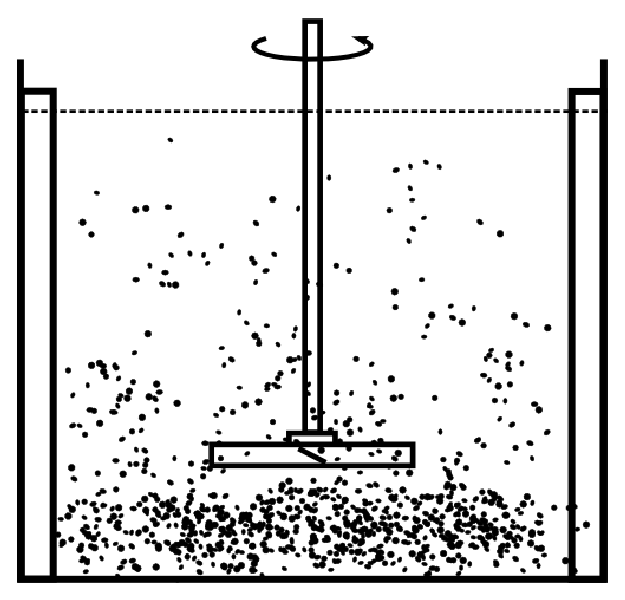
\includegraphics[scale=0.35]{images/typy_suspenzi-1.eps}}
  \qquad
  \subfloat[Úplná]{\label{fig:typ2}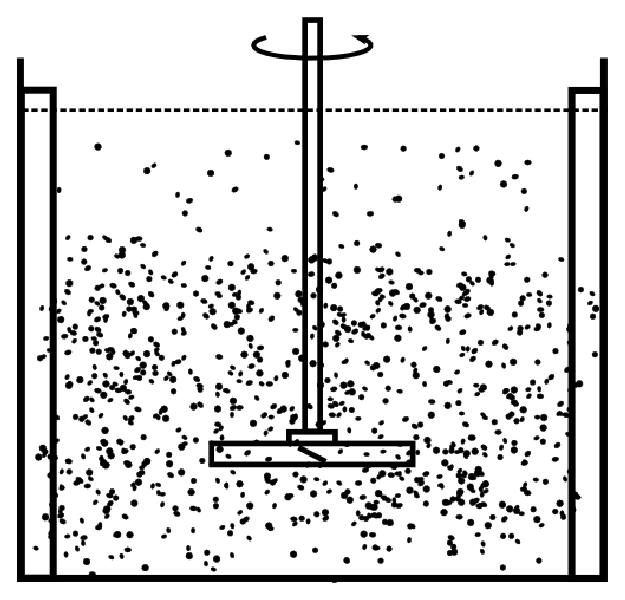
\includegraphics[scale=0.35]{images/typy_suspenzi-2.eps}}
  \qquad
  \subfloat[Homogenní]{\label{fig:typ3}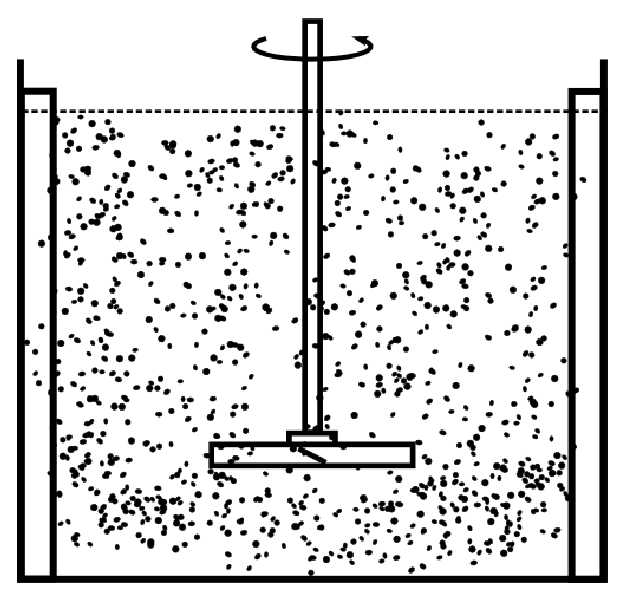
\includegraphics[scale=0.35]{images/typy_suspenzi-3.eps}}
  \caption{Stupně suspendace}
  \label{fig:typsus}
\end{figure}

Při částečné suspendaci lze vizuálně pozorovat pohyb částic pevné fáze pouze v blízkosti dna nádoby. Toto shlukování má za následek zhoršení přestupu tepla a hmoty, což v důsledku může snížit rychlost probíhajících chemických reakcí. Z výše uvedeného vyplývá, že podmínky částečné suspendace jsou postačují pouze při míchaní vysoce rozpustných látek.

Stav úplné suspendace je charakterizován pohybem pevné fáze v celé nádobě, přičemž žádná částice nezůstává na dně déle než jednu až dvě sekundy. Tato podmínka se někdy označuje jako Zwieteringovo kritérium podle autora, který jako první na základě experimentů navrhl vztah k výpočtu kritické (minimální) frekvence otáčení míchadla potřebné k dosažení stavu úplné suspendace. Při tomto stavu je maximální povrch částic vystaven kapalině, což má za následek intenzivní transport hmoty a tepla mezi jednotlivými fázemi.

Posledním stádiem je dosažení stavu homogenní suspendace, při němž částice pevné fáze dosahují prakticky rovnoměrného rozložení v celém promíchávaném systému. Jakékoliv další zvýšení frekvence míchadla nebo jeho příkonu nemá již prakticky žádný vliv na distribuci pevné fáze. Dosažení stavu homogenní suspendace je často důležité u procesů, které vyžadují rovnoměrné rozložení částic v systému. Příkladem takovéhoto procesu může být krystalizace, kde nerovnoměrná koncentrace pevné fáze způsobuje tvorbu míst s lokálním přesycením, jenž následně negativně ovlivňují kvalitu vzniklých krystalů. Nicméně ve většině případů je postačující dosažení stavu úplné suspendace, který vyžaduje menší množství vykonané práce.

\subsection{Kritická frekvence otáčení míchadla}
Jak již bylo zmíněno v předcházející kapitole, kritická frekvence otáčení je minimální rychlost otáčení míchadla potřeba k udržení částic pevné fáze ve vznosu. První kdo navrhl empirickou korelaci k jejímu výpočtu byl \citet{zwi58}. Jím navržený vztah má tvar:

\begin{equation}
	N_{js} = \left[\frac{g(\rho_{s}-\rho_{l})}{\rho_{l}}\right]^{\num{0.45}}W^{\num{0.13}}d_{p}^{\num{0.2}}D^{\num{-0.85}}\nu^{\num{0.1}}S
	\label{eq:nkrit}
\end{equation} 

\noindent kde $g$ je gravitační zrychlení, $\rho_{s}$ hustota pevné fáze, $\rho_{l}$ hustota kapalné fáze, $W$ relativní hmotnostní zlomek pevné fáze, $d_{p}$ průměr částice pevné fáze, $\nu$ kinematická viskozita a $S$ je bezrozměrná Zwieteringova konstanta, která zohledňuje geometrii systému a míchadla. Ze vztahu je dobře patrné, že rozdíl hustot jednotlivých fází nejvýznamněji ovlivňuje výslednou kritickou frekvenci otáčení míchadla. Pozdější studie provedené, jenž provedli, 

\newpage 
\section{Počítačová dynamika tekutin (CFD)}



